\chapter{Theoretical background: single-particle dynamics}
This chapter provides the theoretical knowledge on the dynamics of electrons in storage rings needed to acquaint the reader with the online optimization problem and the constraints involved. The main objective is to introduce the linear dynamics theory, the optics functions, the operation parameters such as the tunes and chromaticity and to conceptualize the amplitudes limitations due to the nonlinearities of the motion. This chapter also aims at introducing SIRIUS' operation parameters and specifications. We claim no original contribution. All the content presented here can be found in the accelerator physics and engineering literature, in particular, refs.~\cite{sands_physics_1969,lee_accelerator_2004,wiedemann_particle_2015,wolski_beam_2014}.

Despite the complicated physics of fully-coupled dynamics involving transverse, longitudinal awe have already examined in section effects and instabilities, for the purpose of this dissertation and the optimization problem at sight, we model the motion of a single electron, neglecting radiation losses and gains and any other collective interactions. These simplifications are justified for our immediate purposes because:
\begin{itemize}
    \item The beam is injected into the storage ring on-energy: it has no significant energy deviations and thus it does not perform large energy and longitudinal oscillations once it is captured into the ring;
    \item radiation losses are only significant over a time scale of a couple of turns. Over this period, tens of transverse oscillations take place. A model neglecting losses is relatively accurate for a small number of turns soon after the injection;
    \item the linear and uncoupled dynamics this simpler modeling renders serves as an initial building block upon which elaborate modeling can be carried out, incorporating coupling, nonlinearities and perturbations, as well as collective effects;
\end{itemize}
In this simplified picture, the electron travels along the ring at the speed of light and executes transverse oscillations in two orthogonal planes. The dynamics takes place in a 4-dimensional phase space, identical to that of two independent quasi-periodic oscillators.

\section{Motion of charged particles in magnetic fields}
\subsection{Circular cyclotron motion}
An electron of charge $e$ and momentum magnitude $p$ follows a circular orbit of radius $\rho$ when interacting with an uniform and time-independent magnetic field of magnitude $B$, directed perpendicularly to the orbit plane. In such conditions, the Lorentz force law predicts that the orbit radius reads
\begin{equation}
    \rho = \frac{p}{Be}.
    \label{eq:Lorentz}
\end{equation}
Rearranging this relation we can define a quantity with units of magnetic field~$\times$ length which characterizes the momentum magnitude per unit charge of the beam, the \textit{magnetic rigidity}:
\begin{equation}
    R(p) \equiv B\rho = \frac{p}{e}.
    \label{eq:rigidity}
\end{equation}
\subsection{Trajectory deflections}
\begin{figure}[htb]
    \centering
    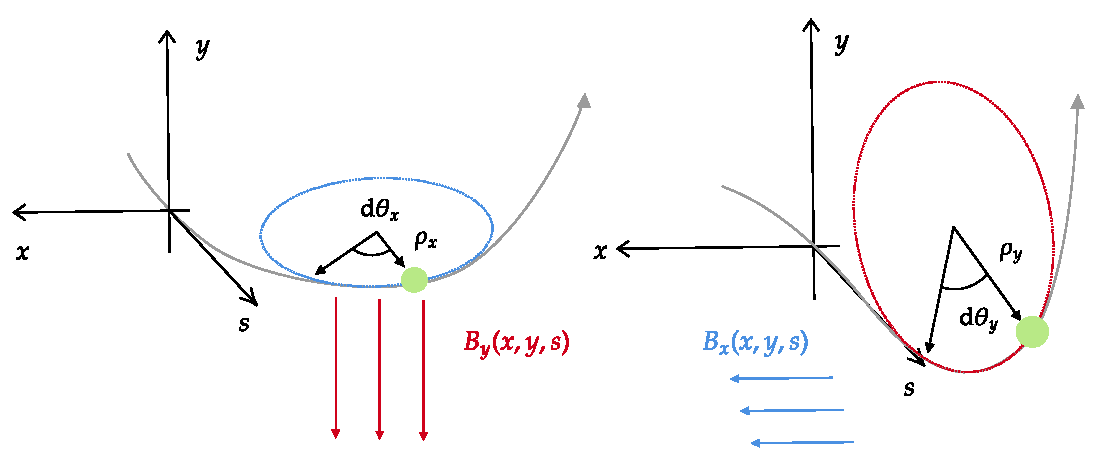
\includegraphics[width=\textwidth]{Images/deflections.pdf}
    \caption[Illustration of trajectory deflection when interacting with magnetic fields.]{Illustration of trajectory deflection when interacting with magnetic fields.}
    \label{fig:deflec_angles}
\end{figure}
Consider an electron traveling along a curve parameterized by the arc-length $s$ with respect to an arbitrary reference point. Define the normal and bi-normal unit vectors so that we can identify a $x-y$ plane perpendicular to the motion.  Let $B_x(x,y,s)$  and $B_y(x,y,s)$, denote the magnetic field components along the unit vectors. The interaction with the fields results in deflections of the trajectory, whose deflection angles $\dd\theta_u$ in the $u=x,y$ plane can be estimated from the local curvature radius $\rho_u$ and infinitesimal displacement $\dd{s}$ with the aid of a local, instantaneous version of equation~\eqref{eq:Lorentz}:
    \begin{equation}
        \begin{aligned}
            \dd{\theta_u} & = \frac{\dd{s}}{\rho_u(s)} = \frac{e}{p}B_v(x,y,s)\dd s = \frac{1}{R(p)}B_v(x,y,s)\dd s, \quad u,v=x, y \quad\text{or}\quad y,x.
        \end{aligned}
        \label{eq:deflec_angles}
    \end{equation}
Where eq.~\eqref{eq:rigidity} has been used to identify the $p/e$ ratio as the magnetic rigidity $R(p)$. These considerations are illustrated in Fig.~\ref{fig:deflec_angles}. The rigidity depends solely on the electron's momentum/energy and serves as the appropriate normalization constant to evaluate the instantaneous angular deflections in the electron's trajectory caused by magnetic fields.
\section{The coordinate system for storage ring dynamics}
As sketched by Fig.~\ref{fig:storage_ring}, electrons in a storage ring perform oscillations close to a nearly circular reference closed orbit. A convenient coordinate frame to describe the dynamics in this scenario can be constructed by imagining a reference particle traveling along a curve drawn by the tip of a vector $\vb{r}_0$, as Fig.~\ref{fig:frenet-serret} shows. This particle samples exactly the reference nominal orbit and travels a distance $s$ along the ring, which can be used to parameterize the motion. The triad of direction vectors for the co-moving coordinate frame consists of the vector $\vu{s}$, tangent to the trajectory, the vector $\vu{x}$, normal to the trajectory, pointing in the direction at which $\vu{s}$ changes, and a vector $\vu{y}=\vu{x}\cross\vu{s}$, bi-normal to the trajectory. This construction leads to a Frenet-Serret reference frame.

Assuming no curvature in the $y$ plane, i.e. that the accelerator defines a curve whose plane is parallel to the facility flat floor, then the tangent, normal and binormal unit vectors defining the frame can be calculated as \cite{lee_accelerator_2004}
\begin{equation}
\vu{s}=\dv{\vb{r}_{0}}{s}, \quad \vu{x}=-\rho\dv{\vu{s}}{s}, \quad \vu{y} =  \vu{x}\times\vu{s},
\end{equation}
where $\rho(s) = \norm{\dv*{\vu{s}}{s}}^{-1}$ is the local curvature radius\footnote{For a circular trajectory, $\vb{r}_0 = \mqty[R\cos(s/R) & R\sin(s/R) & 0]^\intercal$, $ 0\leq s \leq L$, in the laboratory frame. So we can calculate $\vu{s}=\mqty[-\sin(s/R) & \cos(s/R) & 0]^\intercal$, $\dv*{\vu{s}}{s} = -R^{-1}\mqty[\cos(s/R) & \sin(s/R) & 0]$, which reveals $\rho(s)=R$, justifying the interpretation of $\rho(s)$ as a curvature radius.}. The vectors evolve along $s$ as prescribed by the Frenet-Serret equations:
\begin{equation}
\dv{\vu{s}}{s}=-\frac{1}{\rho(s)}\vu{x}, \quad\dv{\vu{x}}{s}=\frac{1}{\rho(s)}\vu{s}, \quad \dv{\vu{y}}{s}=0.
\end{equation}
The frame depends solely on the geometry of the specified path: the instantaneous curvature $\rho^{-1}(s)$. Since the curvature is defined by the strengths of the dipolar fields $B_0(s)$ in the $y$ direction, then, eq.~\eqref{eq:deflec_angles} leads to1. Theoretical background: single-particle dynamics
    \begin{equation}
        \frac{1}{\rho(s)} = \frac{B_0(s)}{R_0},
        \label{eq:G}
    \end{equation}
where $R_0$ is the rigidity of the beam at the nominal energy.
%As a starting point for designing the magnetic lattice of an accelerator, given the desired energy range for the beam and its rigidity and the desired radius of curvature, the required integrated strength of the dipoles must satisfy the above relation.

The transverse deviations from the nominal orbit can be measured in units of the unit vectors $\vu{x}$, $\vu{y}$ in the normal and bi-normal directions. These deviations characterize the transverse dynamics of the electron. One may also be concerned with the distance of a given particle from the reference particle along the curve. Such differences arise due to differences in the energy of two particles. In the full, six-dimensional dynamics, the longitudinal distance from the reference particle and the energy deviations are conjugate dynamical variables characterizing the longitudinal dynamics. They typically oscillate within a range of stable values, characterizing the energy acceptance. As mentioned above, since no radiation loss nor gain will be considered in our modeling, the energy and longitudinal deviations from the reference particle shall be static and treated as fixed parameters.

\begin{figure}[htb]
    \centering
    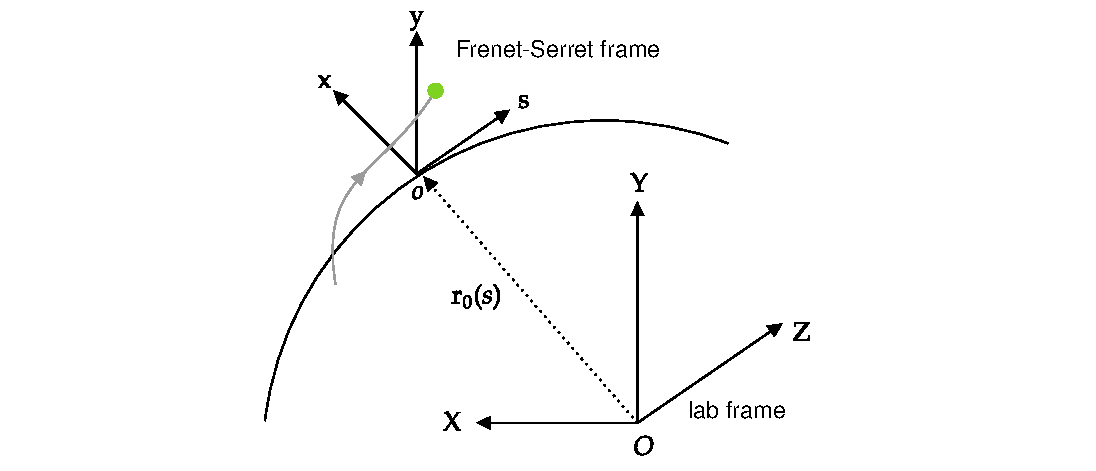
\includegraphics[width=0.9\textwidth]{Images/frenetserret.pdf}
    \caption[The Frenet-Serret coordinate system]{The Frenet-Serret coordinate system. Figure inspired by ref.~\cite{huang_beam-based_2019}.}
    \label{fig:frenet-serret}
\end{figure}

\section{Hamiltonian for the relativistic electron}
The dynamics of relativistic electrons influenced by electromagnetic fields $(\Phi, \vb{A})$ is encapsulated by the Hamiltonian \cite{landau_classical_1975}
    \begin{equation*}
        H=\sqrt{m^2c^4+(\vb{P}-q\vb{A})^2c^2}+e\Phi,
    \end{equation*}
 $e$ being the elementary charge and $\vb{P}=\vb{p}+e\vb{A}$ the canonical momentum, with $\vb{A}$ being the vector potential describing the magnetostatic fields of the lattice, i.e. $\vb{B}=\curl \vb{A}$. To obtain equations of motion for electrons in the storage ring, one usually follows the steps below:
 \begin{itemize}
    \item A canonical transformation to change coordinates is applied in order to describe the motion in terms of the Frenet-Serret frame variables $x$, $y$;
    \item Instead of time $t$, the Hamiltonian and the dynamical variables are described as functions of $s$, the longitudinal position along the ring;
    \item Paraxial approximation: the transverse momenta are assumed to be way smaller than the momentum along the trajectory's tangent direction. This allows the expansion of the square-root in the Hamiltonian as a power series, revealing the expression for an approximate Hamiltonian, which can be more easily handled;
    \item Geometric quantities are used: in the paraxial approximation, the canonical momenta for on-energy particles are identified with the derivatives with respect to the parameter $s$, i.e., $p_x = x^\prime = \dv*{x}{s}$ and $p_y = y^\prime = \dv*{y}{s}$, which represent the divergence angles from the nominal orbit. For off-energy particles, a correction factor is present;
 \end{itemize}
 All of the transformations and manipulations summarized above can be found in detail in the literature, such as in Refs.~\cite{lee_accelerator_2004, wiedemann_particle_2015,  wolski_beam_2014}. As mentioned previously, by neglecting RF cavities ($\Phi=0$) and radiation losses, the energy will be a constant parameter, and the dynamics will consist solely of the transverse degrees of freedom.  In this 4-dimensional dynamics, the set of canonical variables are $(x,p_{x},y , p_{y})$, where the momenta are given by
\begin{equation} p_{x}= x^\prime(1+\delta),\quad p_{y}=y^\prime (1+\delta)\end{equation}
and $\delta$ is the relative deviation from the nominal energy-momentum:
\begin{equation}
    \delta \equiv \frac{P-P_{0}}{P_{0}}\approx\frac{E-E_0}{E_0}.
\end{equation}
The ultra-relativistic approximation $E\approx pc$ was used. For on-energy particles, $p_x = x^\prime$, $p_y = y^\prime$.

Hamilton's equations for the paraxial-approximated Hamiltonian reveals the equations of motion for the $x$ and $y$ coordinates, which read:
\begin{equation}
x^{\prime \prime}=-\frac{(1+G x)^{2}}{1+\delta} \frac{B_{y}}{R_0}+G(1+G x),
\quad
y^{\prime \prime}=\frac{(1+G x)^{2}}{1+\delta} \frac{B_{x}}{R_0},
\label{eq:EOMs}
\end{equation}
where $R_0 = p_0/e$ is the magnetic rigidity of the beam at the nominal energy and $G(s)\equiv\rho^{-1}(s)$ is the inverse local radius of curvature, related to the dipole fields as in Eq.~\eqref{eq:G}.

\section{The magnetic fields}
To study the motion, we need to specify the fields $B_x(s)$ and $B_y(s)$ acting on the beam. Since in a storage ring the magnets are arranged as periodic arrays of dipoles, quadrupole, and sextupoles, the $B_x(s)$ and $B_y(s)$ functions are generally periodic. The magnetic fields are sectionally defined and have the following functional forms
\begin{itemize}
    \item Horizontal Dipole
           \begin{equation} B_x(s) = 0, \quad B_y(s) = B_0, \quad \text{inside dipoles},
            \label{eq:dipole}
           \end{equation}
    \item Normal quadrupole
          \begin{equation}B_x = B_1 y, \quad B_y = B_1 x, \quad \quad \text{inside quadrupoles},
            \label{eq:quadrupole}
           \end{equation}
    \item Normal sextupole
          \begin{equation}B_x = B_2xy, \quad B_y = \frac{1}{2}B_2(x^2 - y^2), \quad \quad \text{inside sextupoles},
            \label{eq:sextupole}
           \end{equation}
\end{itemize}
and zero everywhere else, in drift sections. Fields \eqref{eq:dipole}--\eqref{eq:sextupole}  are the so-called \textit{normal multipole fields}, in contrast with \textit{skew multipole fields}, which couple the horizontal and vertical dynamics. We will neglect skew fields and coupling for now. They can be treated as perturbations in perturbation theory schemes.

In eqs.~\eqref{eq:EOMs}, the magnetic rigidity normalizes all the fields. Thus, we define the normalized dipolar, quadrupolar and sextupolar field strengths, $G(s), K(s), S(s)$:
\begin{equation}
    G(s) = \frac{B_0(s)}{R_0}, \quad K(s) = \frac{B_1(s)}{R_0}, \quad S(s) = \frac{B_2(s)}{R_0}.
    \label{eq:mag_funcs}
\end{equation}
For a SIRIUS superperiod, the functions are shown in Fig.~\ref{fig:field_funcs}. A superperiod consists of the basic repetition of four magnetic cells. SIRIUS has 5 superperiods. In other words, the curves in Fig.~\ref{fig:field_funcs} repeat themselves five times along the $518~\unit{m}$ of the ring. More details on the magnetic lattice are in section~\ref{sec:mag_latt}.
\begin{figure}[htb]
    \centering
    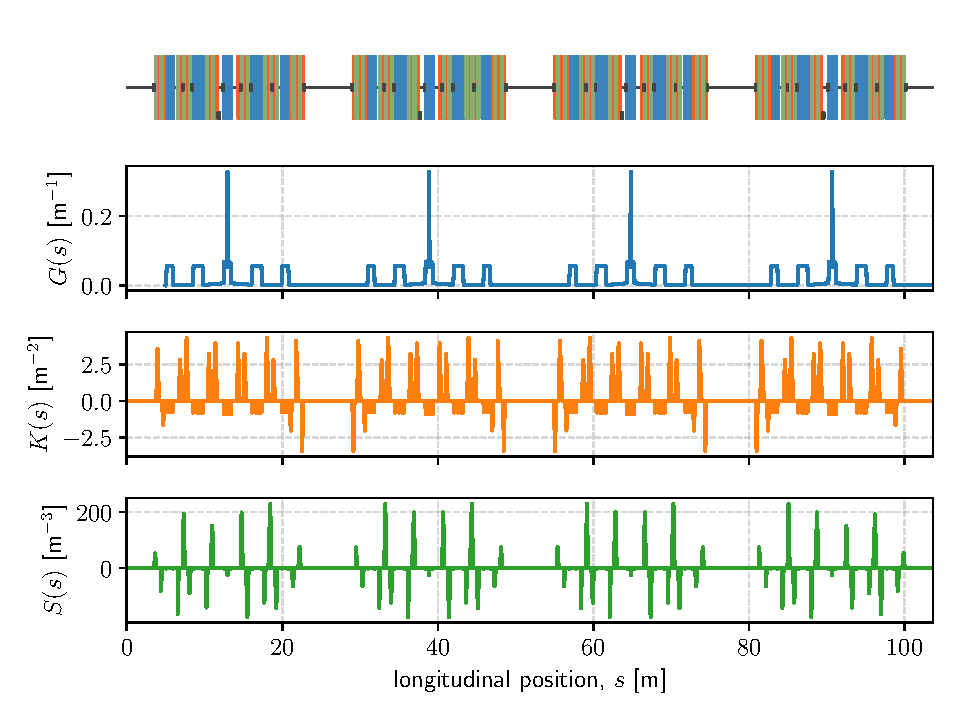
\includegraphics[width=\textwidth]{Images/field_functions.pdf}
    \caption[Normalized field functions for dipoles, quadrupoles and sextupoles of a superperiod of SIRIUS lattice]{Normalized field functions for dipoles (top plot), quadrupoles (middle plot) and sextupoles (bottom plot) of a superperiod of SIRIUS lattice, shown at the top. Colored blocks represent the magnets of the accelerator lattice: blue for dipoles, orange for quadrupoles and green for sextupoles. The ring has a 5-fold symmetry, with the cells, fields, and optics function repeating the pattern shown above five times up to $s=518~\unit{m}$.}
    \label{fig:field_funcs}
\end{figure}
\section{Linear dynamics}
Expansion of eqs.~\eqref{eq:EOMs} up to first order in the $x, y, \delta$ variables leads to \cite{sands_physics_1969}
    \begin{equation}
        x^{\prime\prime}+(G^2+K)x=G\delta, \quad
        y^{\prime\prime}-Ky=0.
        \label{eq:linearEOM}
    \end{equation}
    For on-momentum particles, $\delta=0$, both equations are instances of Hill's equations
    \begin{equation}
        u^{\prime\prime}+K_u(s)u = 0,
        \label{eq:Hill}
    \end{equation}
   i.e, a pair of parametric oscillators for $u=x,y$, with $s$-dependent and periodic focusing functions
         $$K_x(s) = G^2(s) + K(s), \quad K_y(s) = - K(s),$$
    the analogs to an oscillator's spring force per unit mass. Motion in the linear approximation thus consists of oscillations around the closed orbit, known as \textit{betatron oscillations}.
\subsection{Pseudoharmonic description}
Betatron motion can be cast in an amplitude-phase form. One can show that
\begin{equation}
    u(s) = \sqrt{2\beta_u(s) J_u}\cos(\phi_u(s) + \phi_0),\quad u=x,y,
    \label{eq:pseudo_harmon}
\end{equation}
is a solution to \eqref{eq:Hill}, as long as the $\beta_u(s)$ function satisfies the boundary-value problem
\begin{equation}
    \frac{1}{2}\beta_{u}^{\prime\prime}+\beta_{u} K_u(s) - \frac{1}{\beta_{u}}\qty(\frac{1}{4}\beta_{u}^{\prime 2} + 1 ) = 0, \quad
        \begin{cases}
            \beta_{u}(0) = \beta_{u}(L)\\ \beta_{u}^{\prime}(0) = \beta_{u}^{\prime}(L)
        \end{cases}
    \label{eq:beta_eq}
\end{equation}
and the phase advance is given by
    \begin{equation}
        \phi_u(s) = \int_{0}^{s}\frac{1}{\beta_u(\sigma)}\dd\sigma.
   \end{equation}
The motion is oscillatory, non-harmonic, and non-periodic. The oscillations envelope is the square root of the beta functions $\beta_u(s)$, which for the SIRIUS storage ring are shown in Fig.~\ref{betafunc}.
\begin{figure}[htb]
    \centering
    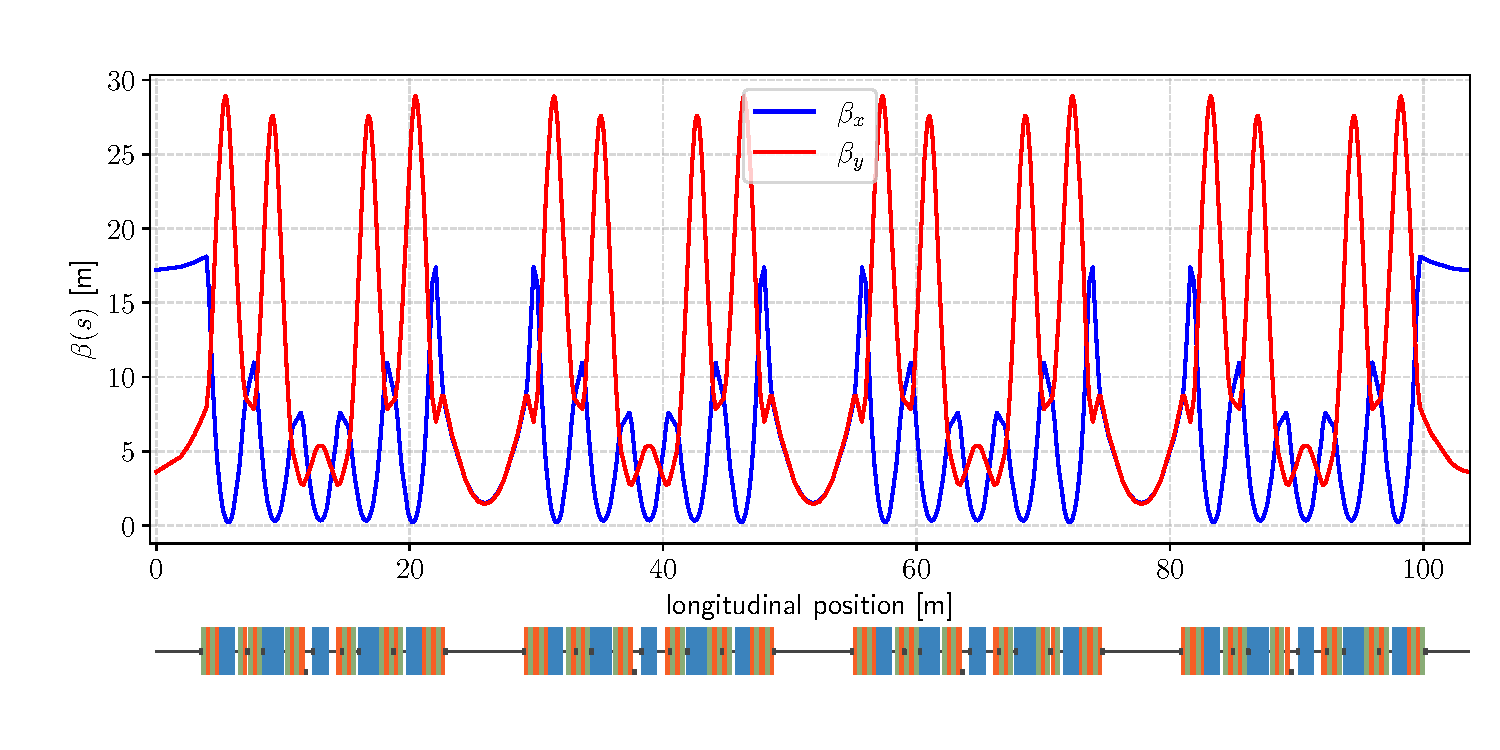
\includegraphics[width=\textwidth]{Images/beta_functions.pdf}
    \caption[Betatron functions in a superperiod of the SIRIUS storage ring]{Betatron functions in a superperiod of the SIRIUS storage ring.}
    \label{betafunc}
\end{figure}
\subsection{The tune}
An important parameter of the dynamics is the \textit{tune}: the phase advance over a revolution along the ring, in units of a complete cycle:
\begin{equation*}
    \nu_u=\frac{1}{2\pi}\int_{s}^{s+L}\frac{\dd \sigma}{\beta_u(\sigma)}\equiv\frac{1}{2\pi}\oint\frac{\dd s}{\beta_u(s)}.
\end{equation*}
The tune reveals the number of transverse oscillations per revolution along the ring. The optimized tunes during design phase for SIRIUS storage ring are $(\nu_x, \nu_y)=(49.08, 14.14)$. These were the machine tunes prior to this work.

When studying the effects of perturbations and nonlinearities acting on the beam, one realizes that tunes are critical variables in determining the beam's response. More specifically, the tunes impact over disturbances amplification factors, which are greatest when tunes are close to integer numbers. Ideally, it is desired for the tunes to be far from the integers, but also far from the half-integers. We examine the relation between the tunes and the effects of disturbances in more detail in section \ref{sec:field_err}.

\subsection{Turn-by-turn motion}
If one keeps track of the time evolution of the $u, u^\prime$ variables at a fixed position along the ring, plotting them in a phase space, one realizes the quasi-periodic motion traces out ellipses. This fact can be analytically verified by calculating the derivative
    \begin{equation}
        u^{\prime}(s) = - \sqrt{\frac{2J_u}{\beta_u}}\qty[\sin(\phi_u(s) + \phi_0) - \frac{1}{2}\beta_u^\prime(s)\cos(\phi_u(s) + \phi_0)],
        \label{eq:uprime}
    \end{equation}
    defining the functions $\alpha_u = -\frac{\beta_u^\prime}{2}$  and $\gamma_u = \frac{(1+\alpha_u^2)}{\beta_u}$ and checking that $u, u^\prime$ satisfy the quadratic form
    \begin{equation}
        2J_u=\gamma_u u^{2}+2\alpha_u u u^{\prime}+\beta_u u^{\prime2},
     \end{equation}
which describes the ellipse. The ellipse properties are determined by the $\beta_u(s), \alpha_u(s)$ and $\gamma_u(s)$ functions, also known as Courant-Snyder (C-S) parameters or Twiss parameters, as Fig.~\ref{fig:ellipse} shows. Since the parameters are functions of the position $s$, then, at each point along the accelerator, the Poincaré Section $u, u^\prime$ displays a different ellipse. Although different in shape, their areas are proportional to $J_u$, an invariant quantity determined by the particle's initial condition. The ellipse areas are thus conserved along the ring \cite{lee_accelerator_2004,wiedemann_particle_2015}.

 Since the phase advance over a turn is $2\pi \nu+\phi_0$, the phase advance after the $j$-th turn is $2\pi\nu j+\phi_0$, and thus
 sampling the transverse motion at a fixed $s=s_0$ position reveals a harmonic displacement, which at the $j$-th turn reads
\begin{equation}
    u_j(s_0)=\sqrt{2\beta_u(s_0) J_u}\cos(2\pi\nu_u j+\phi_u(s_0)).
    \label{eq:TbT_motion}
\end{equation}
Knowledge of this formula allows the determination of the tunes (mod $2\pi$) from the observation of \gls*{tbt} motion of the beam. The time-series of positions can be fitted to eq.~\eqref{eq:TbT_motion} in the time domain, or the signal can be processed in the frequency domain for the identification of the harmonic corresponding to $\nu_u$.
% Time of flight during a complete turn is $L/c$ so, for the $j$th turn, $t_j=\frac{L}{c} j$. With a revolution frequency of $\omega_r=2\pi/(L/c)$, we see that $2\pi j= \omega_r t_j$. As a function of the time elapsed over the $j$ turns, the displacements reads
% \begin{equation}
%     x_j=\sqrt{2\beta_0J}\cos(\omega_r\nu t_j+\phi_0).
% \end{equation}
\begin{figure}[htb]
    \centering
    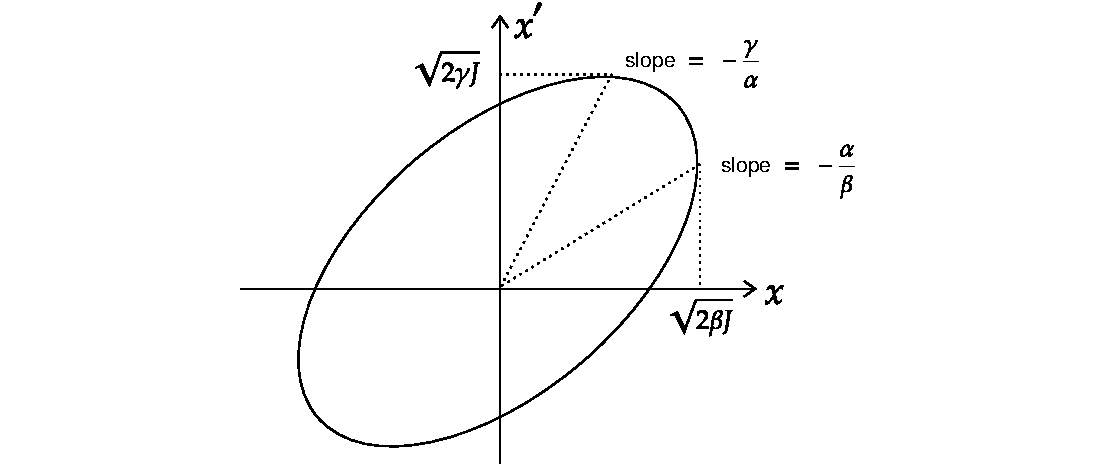
\includegraphics[width=0.9\textwidth]{Images/ellipse.pdf}
    \caption[Ellipse traced by TbT motion in the $(x,x^\prime)$ phase space.]{Ellipse traced by \gls*{tbt} motion in the $(x,x^\prime)$ phase space. Optics functions $\alpha(s), \beta(s), \gamma(s)$ determine the principal axes aspect-ratio and the ellipse inclination at each longitudinal position along the ring. Figure inspired by ref.~\cite{wolski_beam_2014}.}
    \label{fig:ellipse}
\end{figure}
\section{Dispersive \& chromatic effects and linear perturbations}
\subsection{Dispersion}
The equation of motion for off-momentum particles in the horizontal plane, the first of eqs.~\eqref{eq:linearEOM}, is a non-homogeneous Hill's equation. The solution consists of the linear combination of the homogeneous solution (betatron motion) and the particular solution: $x=x_\beta+ x_\delta$, which represents an additional deviation from the nominal orbit. Since the non-homogeneous term, $G(s)\delta$, is proportional to $\delta$, we can assume  $x_{\delta} = \eta(s)\delta$, where $\eta(s)$ is the \textit{dispersion function}. For this to be the solution, the dispersion should satisfy
    \begin{equation*}
        \eta^{\prime\prime}+(G^2+K)\eta=G,\quad
        \begin{cases}
            \eta(0) = \eta(L),\\
            \eta^\prime(0) = \eta^\prime(L).
        \end{cases}
    \end{equation*}
    The periodicity in the $\eta(s)$ function is required if we want to interpret it as a closed orbit distortion per relative momentum deviation. Thus, off-momentum particles perform betatron oscillations around a dispersive orbit, displaced from the nominal orbit by $\eta(s)\delta$. The dispersion function for the SIRIUS storage ring is shown in Fig.~\ref{dispersion_func}
    \begin{figure}[htb]
        \centering
        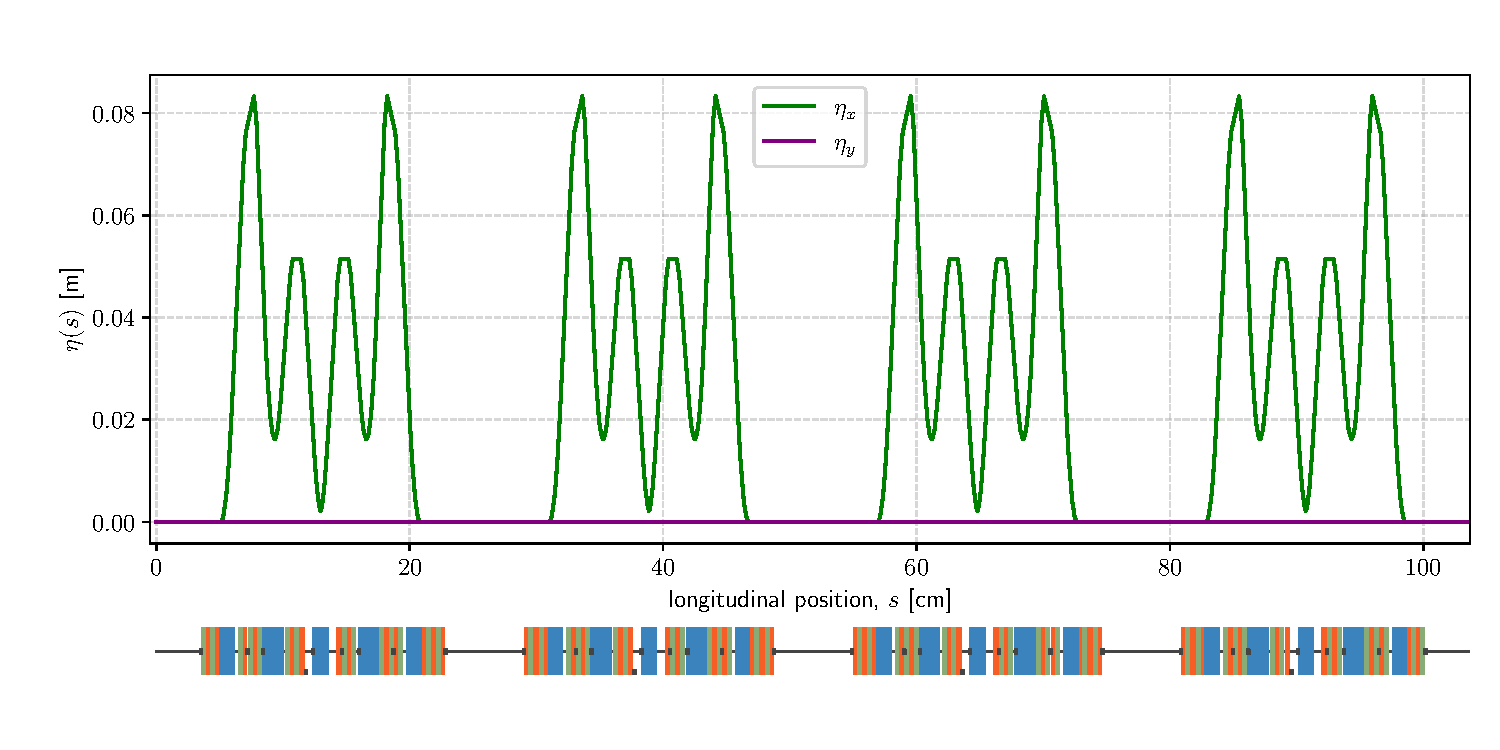
\includegraphics[width=\textwidth]{Images/dispersion.pdf}
        \caption[Dispersion function for a SIRIUS superperiod.]{Dispersion fucntion for a SIRIUS superperiod.}
        \label{dispersion_func}
    \end{figure}
\subsection{Linear Field Errors}
\label{sec:field_err}
    % The dipolar contributions promote additional bendgin and thud disturb the design orbit. Assuming the perturbations are not strong enough to kill the beam, a distorted closed orbit must exist. To find it we need to find the coordinates along the ring which are mapped to themselves after a complete revolution. That is, we must find the fixed point $\vb{X}_{\text{co}}$ of the disturbed one-turn map:
    % \begin{equation}
    %     \vb{X}_{\text{co}} = \mathbf{M} \vb{X}_{\text{co}} + \boldsymbol{\Delta}
    % \end{equation}
    % where $\boldsymbol{\Delta} = (0, \theta)^\intercal$, $\theta = B_y \Delta s / B\rho$ for the $(x, x^\prime)$ slice of the closed orbit, $\theta = B_x \Delta s / B\rho$ for the $(y, y^\prime)$. Solving for the closed orbit we find
    % \begin{equation}
    %     \vb{X}_{\text{co}} = (\mathbf{I} - \mathbf{M})^{-1}\boldsymbol{\Delta}.
    % \end{equation}
    % Using the Courant-Snyder parametrization for the one-turn map at the point $s_0$ immediately downstream the perturbation leads to
    % \begin{equation}
    %     \vb{X}_\text{co} = \frac{\theta}{2\sin\pi\nu}\mqty(\beta_0 \cos\pi\nu \\ \sin\pi\nu - \alpha_0 \cos\pi\nu).
    % \end{equation}

In the presence of additional dipolar and quadrupolar fields representing field errors and deviations from the nominal fields, the orbit and focusing of the beam are changed. Assuming these are small perturbations and not sufficiently strong to perturb the beam severely, we can evaluate the disturbances to the unperturbed dynamics with a simple perturbation theory scheme. The details and derivations can be found in the literature, such as in chapter 2 of Ref. \cite{lee_accelerator_2004}. Here we highlight the main results.
\subsubsection{Dipole errors}
    Suppose there are additional dipole fields $\Delta B_{0x}(s), \Delta B_{0y}(s)$ interacting with the beam other than the dipole fields of the nominal lattice. These translate into errors of the dipolar functions: $\Delta G_y(s)=-\Delta B_{0x}(s)/R_0$ and $\Delta G_x(s)=\Delta B_{0y}(s)/R_0$. In this scenario, the equations of motion read
    \begin{equation}
        x^{\prime\prime}+K_x(s)x=G\delta + \Delta G_x(s), \quad
        y^{\prime\prime}+K_y(s)y = \Delta G_y(s).
        \label{eq:dip_errEOM}
    \end{equation}
    The solution consists of the combination of the betatron motion and the dispersive orbit (for the horizontal plane) plus the closed orbit distortion $u_{\text{co}}$ induced by the additional bending terms due to the dipole errors. For a single thin bending error $\Delta G_u$ in the $u=x,y$ plane, acting for a length $\Delta s$ around $s=s_0$, the closed orbit distortion $u_{\text{co}}$ reads
    \begin{equation}
        u_{\text{co}}(s) = \frac{\sqrt{\beta_u(s)\beta_u(s_0)}}{2\sin\pi\nu_u}\Delta G_u\cos( \pi\nu_u - |\phi_u(s)-\phi_u(s_0)|)\Delta s.
        \label{eq:cod}
    \end{equation}
    For a distribution $\Delta G_u(s)$ of dipolar perturbations along the ring, we sum over the contributions:
    \begin{equation}
        u_{\text{co}}(s) = \frac{\sqrt{\beta_u(s)}}{2\sin\pi\nu_u}\int_{s}^{s+L} \Delta G_u(\sigma)\sqrt{\beta_u(\sigma)}\cos(\pi\nu_u + \phi_u(s) - \phi_u(\sigma))\dd{\sigma}.
        \label{eq:co_dist}
    \end{equation}
    The prefactor involving the sine of the tune shows how $\nu_{u}$ close to an integer can amplify the effects of the dipolar perturbations on orbit distortions. At first, aiming for tunes half-integer tunes $\nu=k/2, k\in\mathbb{Z}$ might seem desirable to minimize the distortions. Choosing so, however, increases the sensitivity to gradient errors, which we examine next.
    % Knowledge of the beam-response to perturbations allows for the inversion of the problem. We can use specified small dipole kicks to correct the orbit, bringing it closer to the nominal one. These small dipole fields are generated by corrector magnets (CM's) abd orbit correction consists on linear problem of seeking CMs strength that minimze orbit distortions.

    % A quadrupole error can be represented by a thin-lens quadrupole transfer matrix \cite{Courant:1958wbj}
    % \begin{equation}
    %     \mathbf{M}_q = \mqty(1 & 0 \\ -k\Delta s & 1),
    %  \end{equation}
    %  so that, immediately downstream the error, the transfer matrix reads $\mathbf{M} = \mathbf{M}_q \mathbf{M}_0$. As a consequence, the optics deviates from the nominal optics. More notouriously, the beta and the phase advances, and thus tune, changes.

    %  The phase advance over a turn, $\phi$, is related to the trace of the one-turn transfer matrix $\mathbf{M}$ as $\cos\phi = 2 \tr \mathbf{M}$. Using the CS parametrization for $\mathbf{M}$, performing the multiplication $\mathbf{M}_q \mathbf{M}_0$ and calcualting the trace leads to
    %  \begin{equation}
    %     \cos \phi - \cos\phi_0 = - \frac{1}{2} k(s)\Delta s \beta_0 \sin\phi_0.
    %  \end{equation}
    %  In a linear approximation (if $\sin \phi_0$ is not near zero) $\Delta(\cos \phi) = \cos \phi - \cos\phi_0 \approx \Delta \phi\dv*{(\cos \phi)}{\phi}$ so the tune-shift due to a single thin-lens quadrupole error is
\subsubsection{Gradient errors}
Gradient errors can be modeled as corrections to the focusing functions in the equations of motion: $K_u(s)\to K_u(s) + \Delta K_u(s)$, for $\Delta K_x(s) = \Delta B_{1y}(s)/R_0$ and $\Delta K_y(s) = -\Delta B_{1x}(s)/R_0$. The changes in beam focusing lead to changes in the beta-functions, phase advances and, consequently, the betatron tunes. One can show the tune-shift as a consequence of a focusing gradient error $\Delta K_u$, acting during a small longitudinal extent $\Delta s$ around $s=s_0$ is \cite{lee_accelerator_2004}
\begin{equation}
    \Delta \nu_u = \frac{1}{4\pi} \beta(s_0) \Delta K_u \Delta s.
    \label{eq:delta_nu}
\end{equation}
Were we dealing with a defocusing error, a minus sign would preceed the above equation. For a distribution of errors we sum over the ring:
\begin{equation}
    \Delta \nu = \frac{1}{4\pi}\oint \beta(s) \Delta K(s) \dd s,
    \label{eq:delta_nu_dist}
\end{equation}
where the closed integration sign refers to a complete circulation along the ring, i.e., integration from $s_0$ to $s_0+L$, for any $s_0\in[0,L)$.

    %  Besides calculating the tune-shift, the resulting transfer-matrix for the lattice with errors allows for the identification of the new optics $\alpha, \beta, \gamma$, which can then be propagated to anywhere in the ring. In particular we can identify $\beta$ and its fractional deviation from the nominal value along $s$, a parameter known as \textit{beta-beating}
    As for the induced error on the beta-functions, it is possible to show that the relative error, known as beta-beat, can be expressed as
     \begin{equation}
        \frac{\Delta \beta_u(s)}{\beta_u(s)} = - \frac{1}{2\sin(2\pi\nu_u)}\int_{s}^{s+L}\Delta K_u(\sigma)\cos[2(\phi_u(\sigma)-\phi_u(s)-\pi\nu)]\dd\sigma.
        \label{eq:beta_beat}
     \end{equation}
which is the largest for $2\nu_u$ closest to an integer. This means we must avoid tunes close to half-integers if we want to avoid the coherent build-up of betatron amplitudes, which can eventually lead to beam loss.
Integer or half-integer tunes are the simplest instances of resonances the beam can be subject to. A more general overview of resonances is presented in subsection~\ref{subsec:resons}.
% \begin{figure}
%     \centering
%     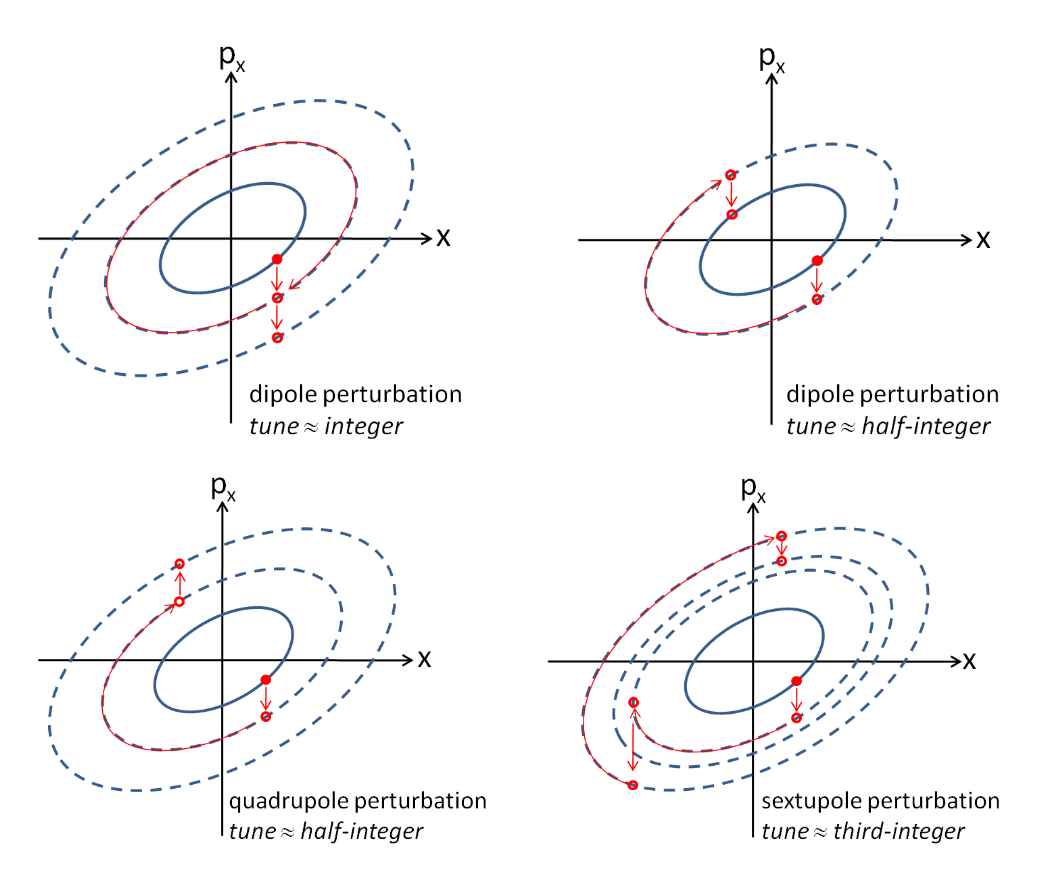
\includegraphics[width=0.6\textwidth]{Images/resonances.png}
%     \caption{!Redo fig: include only dipole and quadrupole! Illustration of phase-space motion under dipolar and quadrupolar perturbations close and away from resonances.}
% \end{figure}
\subsection{Chromaticity}
We have seen how the bending angles at the dipoles are different for electrons with different energies. This is the origin of dispersive orbits. However, energy deviations affect not only the closed orbit by means of the dispersion effect, but also the focusing of the trajectories, since a more/less energetic beam has higher/lower rigidity and thus is focused differently when passing through gradient fields.
%
% As for the higher order effect on the focusing, also known as chromatic effect, we consider the motion in a straight section under a gradient, so that there is no non-homogeneous term in the horizontal equation. The equation of motion considering $x\delta $ terms reads
% \begin{equation}
%     x^{\prime\prime}+(K_x+\Delta K_x)x=0
% \end{equation}
% \begin{equation}
%     y^{\prime\prime}+(K_y+\Delta K_y)y=0
% \end{equation}
% where $K_x=h^2+K_1$, e $K_y=-K_1$ and

Expansion of the equations of motion, eqs.~\eqref{eq:EOMs}, for off-energy particles up to the order of terms $u\delta$ (for $u=x,y$) reveals additional higher-order gradient errors. The focusing functions are corrected by $K_u(s)\to K_u(s) + \Delta K_u(s)$ \cite{lee_accelerator_2004,huang_beam-based_2019}, where
\begin{equation}
    \Delta K_x = -(K+2G^2)\delta \approx - K_x\delta
\end{equation}
\begin{equation}
    \Delta K_y = K\delta = - K_y\delta
\end{equation}
This means there exists an energy-dependent tune-shift effect caused by the gradient error. Using eq.~\eqref{eq:delta_nu_dist}, the tune-shift reads
% The result is that an off-momentum partcile sees a different optics along the ring: different beta function and different phase advance. Thus, it deviates from nominal operation conditions, specially in the tunes, inducing the tune-shifts
\begin{equation}
    \Delta \nu_u = - \frac{1}{4\pi}\oint\beta_u K_u \delta \dd{s},
    \label{eq:energy_delta_tune}
\end{equation}
for the $u=x,y$ planes. We can define the \textit{linear chromaticity} in the $u=x,y$ direction as tune-shift $\Delta \nu_u$ per relative energy deviation $\delta$:
\begin{equation}
    \xi_u=\dv{\nu_u}{\delta}.
\end{equation}
 The chromaticity created by the linear lattice is also called natural chromaticity. Using expression \eqref{eq:energy_delta_tune} for the tune-shift, the natural chromaticity reads
\begin{equation}
\xi_{u, \text {nat }} =-\frac{1}{4 \pi} \oint K_u \beta_u \dd{s}.
\end{equation}

This chromatic aberration effect needs to be corrected to guarantee energy-independent focusing. Correction can be attained with the insertion of sextupolar fields, specifically in the dispersive sections of the storage ring. In such regions, off-energy particles follow a dispersive orbit, and their position reads $x(s)=x_{\beta}(s)+\eta(s) \delta$, where $x_{\beta}(s)$ consists on the betatron oscillations. Since sextupolar fields are of the form
$$B_{x}=B_{2} x y, \quad B_{y}= \frac{B_{2}}{2}(x^{2}-y^{2}),$$
then, the off-momentum particles "see" the fields
$$B_{x}=B_{2}(x_\beta y + \eta \delta y), \quad B_{y}=\frac{B_{2}}{2}({x_\beta^{2}-y^{2}})+B_2 x_\beta \eta \delta + \frac{B_2}{2}(\eta \delta)^2.$$
So, to lowest order in eqs.~\eqref{eq:EOMs}, they feel a dipolar perturbation (which contributes to orbit distortions) and the following gradient perturbation:
$$\Delta K_{x,y}(\delta)=\pm S\eta \delta,$$
recalling that $S(s) = B_2 / R_0$.

Considering the contributions from both the errors induced by energy deviations and also the lowest order sextupole gradient effect, we have a total error of $\Delta K_u = -(K_u \mp S\eta)\delta$ to be inserted in eq.~\eqref{eq:delta_nu_dist}. The chromaticity in a lattice with sextupoles thus reads
\begin{equation}
    \xi_{u}=-\frac{1}{4\pi}\oint\beta_{u}(K_{u}\mp S\eta)\dd{s},
    \label{eq:chromaticity}
\end{equation}
with the minus sign for $u=x$ and the plus sign for $u=y$.

Formula~\eqref{eq:chromaticity} reveals that chromaticity depends linearly on sextupole strengths. This allows for its correction and tuning to desired values. In the SIRIUS storage ring, the operation chromaticity of about $+2.5$ for each plane was determined with the objective of mitigating the transverse instabilities induced by the resistive-wall effect in the range of currents the storage ring is expected to operate: $100$ to $350~\unit{mA}$ \cite[section 7.3]{sa_study_2018}.

 Since a focusing sextupole field focuses in a given plane and defocuses in the other, at least two sextupole families are required for chromaticity correction. To optimize the sextupole strengths required for correction, one family must be placed where $\beta_x > \beta_y$ and another where $\beta_y < \beta_x$. The cost of correcting chromaticity with sextupole is the insertion of nonlinearities in the dynamics. If on the one-hand, amplitude-dependent focusing is needed to correct the energy-dependent focusing (chromaticity), on the other hand it also influence particles with large amplitudes with nonlinearities. To allow for more control over the nonlinear effects and optimization of the dynamics, some families of sextupoles are also placed in non-dispersive sections. They are called achromatic families, since they have no effect over chromaticity up to leading order.
\begin{figure}
    \centering
    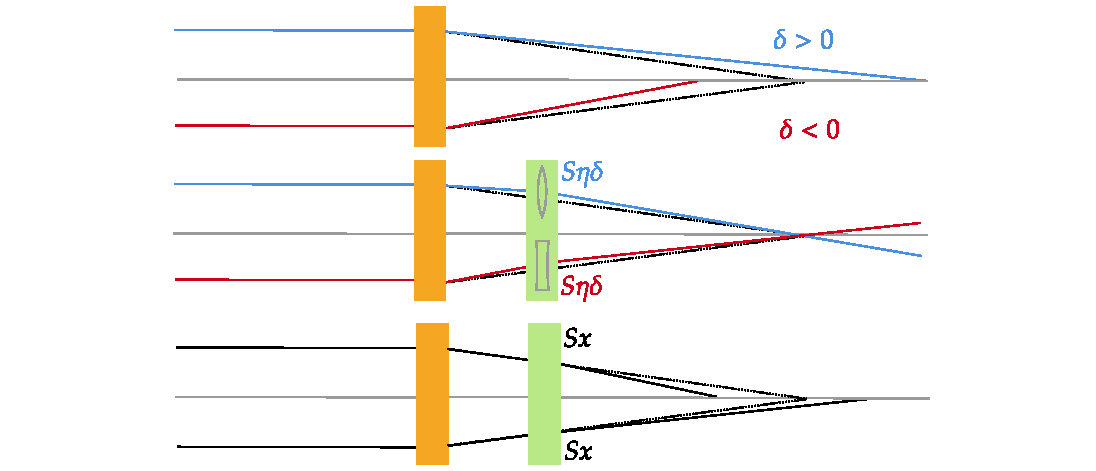
\includegraphics[width=\textwidth]{Images/chromaticity.pdf}
    \caption[Illustration of chromatic aberrations, their correction with sextupoles and examples of geometric aberrations.]{Illustration of chromatic aberrations (top), their correction with sextupoles (middle) and examples of geometric aberrations (bottom).}
    \label{fig:chromaticity}
\end{figure}

\section{Nonlinear dynamics, perturbations, resonances and tune-shifts}
The fields of sextupoles make the dynamics intrinsically nonlinear. To understand the effects of nonlinearities in a generic manner, we develop a basic Hamiltonian perturbation theory in the upcoming sections. However, this requires us to step back momentarily to review linear dynamics in the action-angle variables formalism, upon which we proceed with canonical perturbation theory.
\subsection{Action-Angle Variables}
The betatron equations of motion, Eqs.~\eqref{eq:Hill}, can be obtained as Hamilton's equations for an effective, linear Hamiltonian
\begin{equation}
    \mathcal{H}_u=\frac{1}{2}u^{\prime2}+\frac{1}{2}K_u(s)u^2,
\end{equation}
summed over $u=x,y$.
A transformation $(u,u^\prime)\to(\psi_u, J_u)$ to Action-angle variables is implicitly implemented by the type--1 generating function \cite{lee_accelerator_2004}
\begin{equation}
    F_1(u,\phi_u)=\int{u}^\prime\dd{{u}}=-\frac{u^2}{2\beta_u}\qty(\tan \phi_u-\frac{\beta_u^\prime}{2}).
\end{equation}
The action variable reads
\begin{equation}
    J_u=-\pdv{F_1}{\phi_u} = \frac{u^2}{2\beta_u}\sec^2\phi_u = \frac{1}{2\beta_u}[u^2 + (\beta_u u^\prime + \alpha_u u^2)],
    \label{eq:action}
\end{equation}
from which we can recover the pseudo-harmonic form $u=\sqrt{2\beta_u J_u}\cos(\phi_u(s)+\phi_0)$, and identify the constant $J$ we met before as the action and the betatron phase advance as the angle variable.

In the $J,\phi$ variables, the new Hamiltonian is $H_0(\phi, J)$,  given by
\begin{equation}
    H_u=\mathcal{H}_u+\pdv{F_1}{s} = \frac{J_u}{\beta_u}.
\end{equation}
Performing the change to action-angle variables in both the horizontal and vertical planes, we find the action-angle Hamiltonian for 4D dynamics:
\begin{equation}
    H_0= \frac{J_x}{\beta_x} +  \frac{J_y}{\beta_y}.
\end{equation}
Hamilton's equations read
\begin{equation}
    \phi_u^\prime = \frac{1}{\beta_u(s)},\qquad J_u^\prime=0.
\end{equation}
\subsection{Perturbations and tune-shifts}
Linear motion is integrable since it can be written in terms of the action variable only (angle-independent Hamiltonian). This means the action variable is a constant of motion.

Linear motion, though, is only a useful first approximation. In reality, in a storage ring, there are higher-order multipole magnets, such as sextupole magnets, and also multipole, alignment and excitation errors acting as perturbations. Generically referring to perturbations as the potential $V(J, \phi)$, we can write the perturbed Hamiltonian
\begin{equation}
    H(J,\phi) =H_0 + V(J,\phi),
\end{equation}
For which Hamilton's equations read
\begin{equation}
\phi_u^\prime = \frac{1}{\beta_u(s)}+\pdv{V(J,\phi)}{J_u}, \quad J_u^\prime = -\pdv{V(J,\phi)}{\phi_u}.
\end{equation}
The action is no longer an invariant. It changes as prescribed by the rate of change of the potential with respect to the phase. The phase also changes. The phase advance rate deviates from the linear betatron phase advance, which translates directly into tune-shifts. In this scenario, the tunes depend not only on the momentum, via the chromaticity, but also on the amplitudes (actions). In a general form, we can be express the tunes as
\begin{equation}
    \nu_u = \nu_{u0} + \xi_u(\delta) \delta + \alpha_{uu} J_u + \alpha_{uv} J_v,
\end{equation}
where $\xi_u$ represents the energy-dependent tune-shifts (higher-order generalization of the linear chromaticity), and the other components consist on the amplitude-dependent tune-shifts, up to first order in the actions.
\begin{figure}
    \centering
    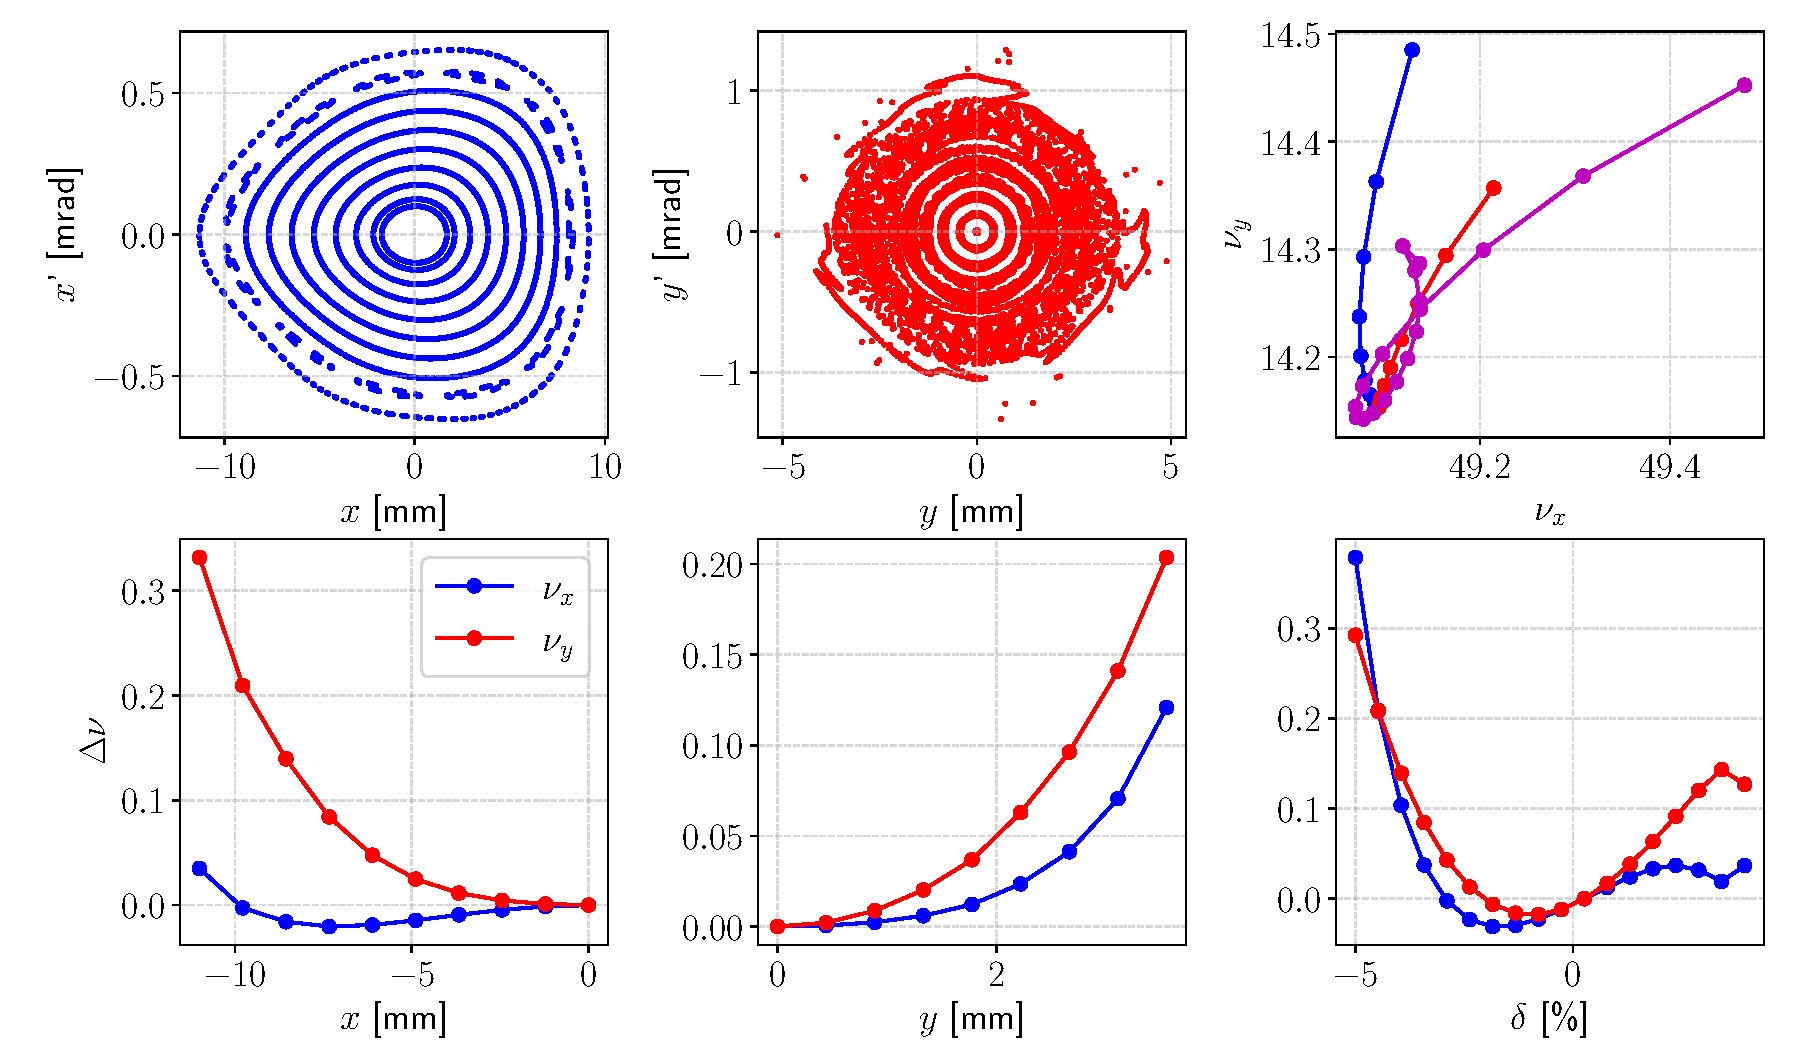
\includegraphics[width=\textwidth]{Images/nonlinear_dynamics_phase_tunes.pdf}
    \caption[Illustration of main characteristics in nonlinear dynamics]{Illustration of main characteristics in nonlinear dynamics. a) \& b): Poincaré sections for motion with increasing horizontal \& vertical amplitudes, respectively; c) Path traced in tune-space for each ellipse of a) in blue, for b) in red, and for each $\delta$ in f), in purple. d) \& e): $x$ and $y$ amplitude-dependent tune-shifts for each ellipse of a) \& b), respectively; f) energy-dependent tune-shifts}
    \label{fig:tune_shifts}
\end{figure}

Figure~\ref{fig:tune_shifts} highlights the main characteristics of the nonlinear dynamics. In a) and b) particles are simulated in SIRIUS' computer model with increasingly larger initial amplitudes in the $x$ and $y$ planes, respectively. The large-amplitude ellipses are distorted, since the action $J$ is no longer an integral of motion. Some large-amplitude particles do not survive. In d) and e), the deviations in horizontal and vertical tunes are shown for the a) and b) simulations, respectively. In d), the tune-shifts in the $y$ and $x$ planes are shown for each initial $x$ amplitude. In e), the tune-shifts for each initial $y$ amplitude in b) is shown. These plots outline the distortion of phase space ellipses, the existence of limiting amplitudes under which regular motion occurs, and the dependence of the tunes with the amplitudes.

In plot e) of Fig.~\ref{fig:tune_shifts}, the chromatic (energy-dependent) tune-shifts are shown: the tune-shifts of particle simulated with energy deviations in the range of $-5\%$ to $5\%$. Linear chromaticity is the derivative of this curve around $\delta=0$. In c), the blue curve represents the path traced in tune-space as the $x$ amplitude increase, i.e., the tunes for each initial condition of the simulations in a); the red curve represents the path traced as the $y$ amplitudes increase,  i.e., the tunes for each initial condition of the simulations in b). The purple curve is the path traced for each $\delta$ in the simulations shown at f).
\subsection{Resonances}
\label{subsec:resons}

4D linear unperturbed motion consists of the motion of two uncoupled parametric oscillators. As a quasi-periodic integrable system, the phase-space is diffeomorphic to the 2-Torus, $\mathbb{T}^2$, and there are an infinite number of such tori covering phase space, corresponding to the different choices of initial conditions $J_u$.

Canonical perturbation theory applied to perturbed motion fails to converge whenever the ratio of tunes is sufficiently rational (resonant tori). The Poincare-Birkhoff theorem states that under such conditions, almost all the periodic phase-space orbits disappear, i.e., almost all the tori are destroyed. An even number of tori survive, half stable and half unstable \cite[section 10.2]{marcus_mecanica2023}. Unstable motion in a storage ring eventually leads to beam loss.

The condition for sufficiently rational tunes, i.e, resonant tori, can be expressed as
\begin{equation}
        m\nu_x + n\nu_y = \ell,
        \label{eq:resonance_condition}
\end{equation}
    for $n, m, \ell\in\mathbb{Z}$. This condition defines lines in tune-space corresponding to the locus in which perturbation theory fails and motion can become unstable: resonance lines.

    We say $|n|+|m|$ is the order of the resonance, which is related to the order of the multipole field perturbation from which it arises.
    %  e.g: order 1 resonances can be driven by dipolar fields, as well as quadrupolar and sextupolar gradients; order 2 can be driven by quadrupolar and sextupolar components; and order 3 can be driven by sextupolar fields.
    Resonances arising from linear field errors, already anticipated in section~\ref{sec:field_err}, are those described by $\nu_x=\ell$ or $\nu_y =\ell, \ell\in\mathbb{Z}$. Normal gradient field errors drive $2\nu_x=\ell$ or $2\nu_y =\ell$ resonances. Skew gradients couple both planes and can drive the famous sum and difference resonances $\nu_x + \nu_y = \ell, \nu_x - \nu_y = \ell$. Sextupoles, up to first-order in perturbation theory, can drive the $3\nu_x=\ell$, resonance, as well as $nu_x \pm 2\nu_y = \ell$ and $\nu_x =\ell$ resonances \cite[section 11.2.4]{wolski_beam_2014}. Figure~\ref{fig:resons} depicts resonance lines in tune-space for resonances up to second, third and fourth order, in the left, middle and right plots, respectively.
\begin{figure}[thb]
    \centering
    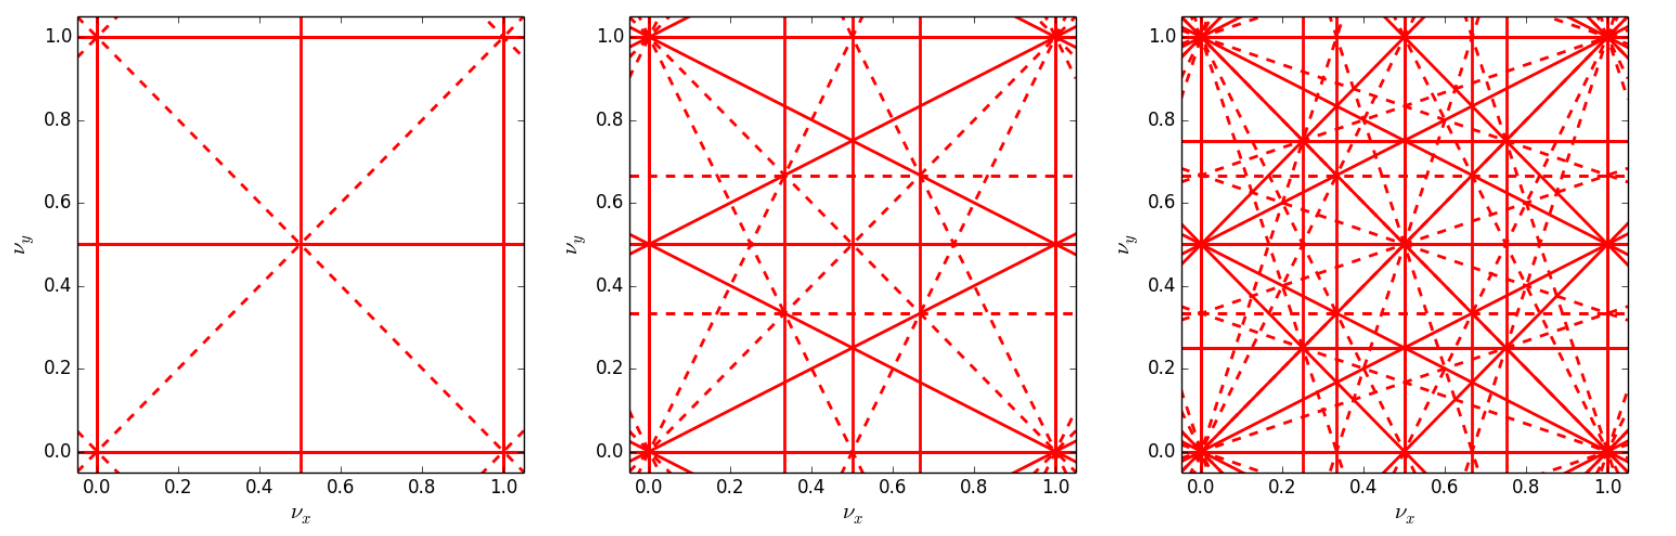
\includegraphics[width=\textwidth]{Images/tunes.png}
    \caption[Resonance lines in tune space up to 2nd, 3rd and 4th order.]{Resonance lines in tune space up to 2nd, 3rd and 4th order, respectively. Solid lines correspond to resonances driven by normal multipole fields, while dashed lines correspond to resonances driven by skew multipole fields. Figure adapted from ref.~\cite{bartosik_first2022}}
    \label{fig:resons}
\end{figure}
\subsection{The Dynamic Aperture}
    The stability of nonlinear dynamics can become sensitive when amplitudes are large. In this scenario, the effects of the nonlinear fields become more significant and the perturbations are dialed up, breaking down the stable tori. Even low-amplitude motion can be dangerous in the long-term due to the phenomenon of Arnold diffusion \cite{wolski_beam_2014, arnold_instability1964}: because of the tune-shifts, especially the amplitude-dependent tune shifts, the tunes can wander in tune space and eventually cross resonance conditions.

    Despite the complexity of predicting stability of nonlinear perturbed dynamics, in electron storage rings, we usually observe the existence of an amplitude limit beyond which instabilities increase and the particles are lost, while the particles below the limiting amplitudes survive. In other words, there are limitations to the maximum transverse amplitudes displaying regular and bounded motion. This behavior was anticipated by the simulations shown in plots a) and b) of Fig.~\ref{fig:tune_shifts} and is also verified in the actual machine during experiments.

The border of the region of stability is the \textit{dynamic aperture} (\acrshort*{DA}). This term can be used to refer to the limiting amplitudes in any of the dynamical variables of phase-space. In this work, we are mostly concerned with the \gls*{DA} in the $(x, x^\prime)$ phase space because of its importance during the beam injection for accumulation into the storage ring.

During injection, if the horizontal amplitudes are larger than the \gls*{DA} along $x$ or $x^\prime$, the beam is not captured efficiently into the storage ring. In this case, increasing the \gls*{DA} to accommodate the incoming beam would be interesting, which is exactly what we aimed at while developing this project.

Since the \gls*{DA} is determined by the nonlinear perturbations, it is possible that tuning the nonlinear fields in a particular manner can render an optimum configuration with increased \gls*{DA}.  In the upcoming chapter, this idea is developed in more detail.
